%%
%% ACM Conference Paper - Converted from TMLR format
%%
\documentclass[sigconf]{acmart}

%%
%% \BibTeX command to typeset BibTeX logo in the docs
\AtBeginDocument{%
  \providecommand\BibTeX{{%
    Bib\TeX}}}

%% Rights management information
\setcopyright{acmlicensed}
\copyrightyear{2025}
\acmYear{2025}
\acmDOI{XXXXXXX.XXXXXXX}

%% Conference information - UPDATE WITH ACTUAL CONFERENCE DETAILS
\acmConference[Conference acronym 'XX]{Conference Title}{Month DD--DD, 2025}{City, Country}
\acmISBN{978-1-4503-XXXX-X/2025/MM}

%% Packages
\usepackage{tikz}
\usepackage{amssymb}
\usepackage{graphicx}
\usepackage{subcaption}
\usepackage{booktabs}
\usepackage[table]{xcolor}
\usepackage{makecell}

\usetikzlibrary{shapes.arrows, positioning, matrix, backgrounds, arrows.meta}
\usetikzlibrary{positioning,arrows.meta,calc,fit,decorations.pathreplacing}

%% Color definitions
\definecolor{WideColor}{HTML}{1B5E20}
\definecolor{longcpColor}{HTML}{8BCAD5}
\definecolor{blueA}{RGB}{33,114,255}
\definecolor{redA}{RGB}{220,53,69}
\definecolor{grayA}{RGB}{140,140,140}

%% TikZ styles
\tikzset{
  dagNodeLinear/.style = {circle, minimum size=7.5mm,
                          inner sep=0pt, font=\footnotesize\bfseries,
                          draw=blue!40!black, very thick, fill=blue!35},
  dagNodeGNP/.style    = {circle, minimum size=7.5mm,
                          inner sep=0pt, font=\footnotesize\bfseries,
                          draw=red!55!black, very thick, fill=red!65!black},
  dagEdgeLinear/.style = {->, line width=1.1pt, draw=black!70, >=Latex},
  dagEdgeGNP/.style    = {->, line width=1.0pt, draw=gray!70, >=Latex},
  dagHalo/.style       = {fill=lightsteelblue!50, draw=none, rounded corners=2pt},
  dagTitle/.style      = {font=\bfseries\small, text=black!75},
}

%%
%% Title and subtitle
\title{On the Role of DAG Structure in Energy-Aware Cloud Scheduling: A GNN-Based Deep Reinforcement Learning Approach}

%%
%% Authors - UPDATE WITH ACTUAL AUTHOR INFORMATION
\author{Anonymous Authors}
\affiliation{%
  \institution{Institution Name}
  \city{City}
  \country{Country}
}
\email{author@institution.edu}

%%
%% Short authors for page headers
\renewcommand{\shortauthors}{Anonymous et al.}

%%
%% Abstract
\begin{abstract}
Cloud providers must assign heterogeneous compute resources to workflow DAGs while balancing competing objectives such as completion time, cost, and energy consumption. In this work, we study a single-workflow, queue-free scheduling setting and consider a graph neural network (GNN)–based deep reinforcement learning scheduler designed to minimize workflow completion time and energy usage.

We identify specific out-of-distribution (OOD) conditions under which GNN-based deep reinforcement learning schedulers fail, and provide a principled explanation of why these failures occur. Through controlled OOD evaluations, we demonstrate that performance degradation stems from structural mismatches between training and deployment environments, which disrupt message passing and undermine policy generalization. Our analysis exposes fundamental limitations of current GNN-based schedulers and highlights the need for more robust representations to ensure reliable scheduling performance under distribution shifts.
\end{abstract}

%%
%% CCS concepts - GENERATE PROPER CODES AT http://dl.acm.org/ccs.cfm
\begin{CCSXML}
<ccs2012>
 <concept>
  <concept_id>10010520.10010553.10010562</concept_id>
  <concept_desc>Computer systems organization~Cloud computing</concept_desc>
  <concept_significance>500</concept_significance>
 </concept>
 <concept>
  <concept_id>10010147.10010257</concept_id>
  <concept_desc>Computing methodologies~Machine learning</concept_desc>
  <concept_significance>500</concept_significance>
 </concept>
 <concept>
  <concept_id>10003033.10003083.10003095</concept_id>
  <concept_desc>Networks~Network resources allocation</concept_desc>
  <concept_significance>300</concept_significance>
 </concept>
</ccs2012>
\end{CCSXML}

\ccsdesc[500]{Computer systems organization~Cloud computing}
\ccsdesc[500]{Computing methodologies~Machine learning}
\ccsdesc[300]{Networks~Network resources allocation}

%%
%% Keywords
\keywords{Cloud Computing, Resource Allocation, Deep Reinforcement Learning, Robustness, Interpretability, Job Scheduling, Graph Neural Networks}

%%
%% Start of document
\maketitle

\section{Introduction}
\label{sec:introduction}

\subsection{Context}

Over the past few years, artificial intelligence and large language models have pushed cloud systems much harder than before. According to \cite{IEA2025DataCenters}, the energy used by data centers keeps growing because of heavier AI training and inference workloads. This means even small improvements in how cloud resources are allocated can save a noticeable amount of time and electricity.

Figure~\ref{fig:Pb definition} shows the setting. A workflow is a directed acyclic graph. Nodes are tasks. Edges are data or control dependencies. Some stages expose wide parallelism. Others form long serial chains. At the same time, machines in a cloud are heterogeneous. Some machines finish tasks faster but draw more power. Others are slower but use less. The scheduler decides, at each step, which ready task should run on which machine. Each assignment changes the makespan and the total energy used.

\begin{figure}[htbp]
    \centering
    \includegraphics[width=\linewidth]{figs/cloud-pb.png}
    \caption{Overview of the workflow scheduling problem in a heterogeneous cloud. The scheduler receives a DAG with ready tasks and a set of machines with different speed and power. It must decide which task runs on which machine, and each choice changes both completion time and energy.}
    \label{fig:Pb definition}
    \Description{Diagram showing workflow DAG scheduling on heterogeneous cloud machines with different speed and power characteristics.}
\end{figure}

This problem has drawn steady research interest. Energy-aware scheduling appeared in HPC and cloud literature well before the recent AI boom. Early work used DVFS to trade performance for power \cite{Zong2007DVFS, Rountree2009DVFS}. Recent surveys report steady activity: Multiple systematic reviews published indicate sustained research activity in this domain \cite{Versluis2020WorkflowSurvey, Ajmera2024VMScheduling}. Machine learning-based cluster management has demonstrated measurable impact, reducing data center energy consumption by up to 15\% in Google's production deployments \cite{GoogleDataCenterAI}. Amazon and Microsoft have explored complementary approaches through right-sizing and spot market mechanisms to reduce both operational costs and resource waste \cite{Cortez2017AWS, Shahrad2020Serverless}.

Modern AI workflows add new dimensions to this problem. They mix layers that are very wide with chains that are very long. And they run on machines with big differences in speed and power use. Old scheduling rules assume the workflow shape stays the same and machines are predictable. When that is not true, performance can drop fast. Because of this, researchers are looking at more advanced schedulers that can adapt. But the problem is we do not know if these learned policies still work when the workflow or machines change. We will go over the current approaches next and then introduce the gap that motivated our study.

\subsection{Related Work}

Many workflow applications are naturally written as directed acyclic graphs (DAGs) of tasks with different resource needs and complex dependencies \cite{deelman2009workflows, sakellariou2010mapping}. Scheduling these DAGs on pools of virtual machines with different speeds and power use is a classic problem in distributed systems and high performance computing \cite{mao2012survey}. This problem is NP hard in general. Foundational work by Pinedo~\cite{Pinedo2012} and the notation of Graham et al.~\cite{Graham1979} provide the standard formal basis for makespan minimization under precedence and machine heterogeneity.

\subsubsection{Classical Structure Aware DAG Scheduling}

A large body of work models applications as weighted DAGs, where nodes are tasks and edges capture precedence and communication constraints on heterogeneous processors. The HEFT and CPOP list schedulers of Topcuoglu et al.~\cite{Topcuoglu2002HEFT} are central references. They rank tasks with path based metrics and map them to heterogeneous processors to reduce makespan. HEFT uses an upward rank that approximates remaining critical path length, then schedules tasks on the processor with the earliest finish time. This exploits DAG depth, fan out, and communication along paths. CPOP identifies a global critical path and assigns its tasks to a single processor to reduce inter processor communication.

Many variants build on this structure aware idea while adding new objectives such as energy or reliability. Energy aware DAG schedulers on heterogeneous and embedded platforms often use critical path and level based slack to decide which tasks can safely be slowed down or consolidated while still meeting deadlines \cite{hu2023online}. In these works, DAG topology is not only a feasibility constraint. It is a direct signal for making decisions. Parallelism per level, critical path length, and slack structure strongly influence task priorities and mapping choices.

In cloud and distributed environments, workflow systems such as Pegasus \cite{Deelman2015Pegasus} and simulators such as CloudSim \cite{Calheiros2011CloudSim} have established DAGs as the standard abstraction for scientific workflows. Energy aware scheduling has been widely studied in this setting. For example, Beloglazov and Buyya~\cite{Beloglazov2012Energy} show how power heterogeneity and task structure together shape good placement policies.

Many real world workloads are also multi objective. Schedulers must trade off makespan, cost, energy, and sometimes reliability \cite{bittencourt2018scheduling, dasilva2017learning}. Classical heuristics are usually tuned around a single dominant objective. When new metrics are added, they often need extensive manual retuning and may not transfer well across workloads \cite{bittencourt2018scheduling}. Meta heuristic methods can explore richer trade offs but are often too slow for real time scheduling in dynamic clouds, since they rely on iterative search \cite{dasilva2017learning}.

\subsubsection{Deep Reinforcement Learning for Resource Scheduling}

These limitations have motivated a shift toward learning based schedulers. Deep reinforcement learning (deep RL), first introduced by Sutton and Barto~\cite{sutton1998reinforcement}, offers a way to learn scheduling policies directly from experience without manually encoding rules for every scenario. Early work by Mao et al.~\cite{mao2016resource} showed that deep RL agents could learn to pack tasks and allocate resources in cluster settings, outperforming hand tuned heuristics on job completion time. The idea is to frame scheduling as a sequential decision problem. An agent observes system state, selects actions such as which task to schedule or which machine to use, and receives rewards based on performance metrics like makespan or resource use.

This approach has several advantages. First, the policy can adapt to patterns in the workload without explicit feature engineering. Second, it can handle multi objective trade offs by shaping the reward function. Third, once trained, the policy can make decisions quickly, which is useful in online settings. Several studies have confirmed that deep RL schedulers can match or beat classical heuristics in controlled environments \cite{zhang2021deepjs, mao2016resource}.

But early deep RL schedulers often treated system state as a flat feature vector. This does not capture the relational structure of workflows or resource topologies. This is where graph neural networks come in.

\subsubsection{Graph Neural Networks for Structured Scheduling}

Graph neural networks provide a natural way to encode relational structure. In scheduling, both workflows (task dependencies) and resource topologies (machine connectivity or hierarchy) are naturally represented as graphs. GNNs use message passing to let each node aggregate information from its neighbors. This means the learned representation can respect the structure of the problem.

Decima was one of the first systems to combine GNNs with RL for cluster scheduling \cite{Mao2019Decima}. It models each data processing job as a DAG of stages. A GNN embeds this DAG along with per stage features such as remaining work and resource demand. The RL policy then uses these embeddings to decide which stage to schedule and how many executors to assign. Message passing over the DAG lets the model implicitly capture properties like depth, critical paths, and fan in or fan out. Experiments showed that this structure aware policy reduced average job completion time compared to structure agnostic baselines and classical heuristics.

Follow up work extended this idea to other scheduling domains. Park et al.~\cite{park2021learning} used GNNs to embed both job DAGs and cluster topology for multi resource scheduling. Others applied similar architectures to workflow scheduling in cloud and edge environments, where tasks have precedence constraints and machines have different speeds or power profiles. In most cases, the GNN based approach improved performance over flat feature representations. These results suggest that exploiting the graph structure provides richer relational information, allowing the policy to generalize more robustly across scenarios.

\subsubsection{Generalization and Robustness Challenges}

Despite these successes, most studies evaluate learned policies primarily on the same types of workflows and host configurations seen during training. They show that GNN based RL can work well in specific settings, but they rarely ask how robust these policies are when the workflow structure or resource characteristics change. For example, what happens when a policy trained on shallow parallel workflows is tested on deep sequential workflows? Or when a policy trained on homogeneous machines is deployed on heterogeneous hardware with conflicting speed and power trade offs?

This concern is grounded in known limitations of graph neural networks under distribution shift. Wu et al.~\cite{wu2022handling} showed at ICLR 2022 that distribution shifts hit GNNs particularly hard because of how nodes connect to each other. When the graph structure changes, the whole representation can break down. This matters for workflow scheduling. A policy trained on one type of DAG may face very different graphs at deployment. Depth can change. Width can change. Branching can change. This motivates a systematic first step: characterize the distribution shift in our setting. We must precisely define and measure how deployment DAGs differ from those seen during training, and then determine how to address it.

\subsection{Positioning of Our Work}

This paper identifies specific out-of-distribution conditions that cause GNN-based deep RL schedulers to fail, and explains why these failures occur.

We build on two key observations. First, Tian et al.~\cite{9460684} showed that real workflows from production systems (millions of DAGs from Alibaba batch jobs) cluster into a few structural types. Second, recent RL-based schedulers using GNNs to embed DAGs have shown strong performance on some benchmarks \cite{Mao2019Decima, park2021learning}, but their robustness across structural types remains unclear.

Our starting point is an empirical pattern reported in Hattay et al.~\cite{hattay2024evaluating}. When a deep RL scheduler is compared with classical heuristics across many workflow instances, it does not simply dominate or fail everywhere. It performs very well on some workflows and host settings and quite poorly on others. Sometimes it is even worse than basic list scheduling rules. With closer examination, we observed that these failures are not random. They concentrate in specific combinations of workflow topology and host heterogeneity. This suggests that learned schedulers have implicit structural domains where they behave coherently and domains where their behavior degrades.

Epistemologically, we follow a Popper style view of scientific progress \cite{popper2005logic}. We are less interested in showing more positive cases for a learned policy and more interested in subjecting it to tests that might break it. We treat the learned policy as a provisional theory about how structure and heterogeneity shape scheduling decisions. We then expose that theory to workflow topologies and host regimes in which it should fail if it is narrow or brittle. The goal is not only to show that the agent can work somewhere, but to reveal what it has actually learned when the surrounding conditions change.

To study this in a controlled way, we define two simple workflow families. \emph{Wide} DAGs are shallow with high parallelism. \emph{Long Critical Path (LongCP)} DAGs have deep dependency chains and little parallel slack. On the resource side, we consider four queue free host regimes that isolate different aspects of heterogeneity: Homogeneous Speed (HS), Homogeneous Power (HP), Aligned (AL), and Non-Aligned (NA). Each regime creates a different trade off between makespan and active energy. As a result, each regime gives a different incentive for using or ignoring parallelism.

We then train a GNN based actor critic deep RL scheduler on these environments. We use separate agents specialized to Wide workflows and to LongCP workflows. We do not evaluate these agents only on the distributions they were trained on. Instead, we systematically probe cross structure and cross regime generalization. For example, we run a Wide trained agent on LongCP workflows, a LongCP trained agent on Wide workflows, and we test all agents across all four host regimes.

This work therefore investigates how DAG topology and host heterogeneity together shape the behavior and generalization of an RL based scheduler with joint energy and makespan objectives in a queue free, single workflow cloud setting.

\paragraph{Research Questions}

This setup lets us ask three main questions:

\begin{itemize}
    \item \textbf{Q1:} How do DAG structure (Wide vs. long critical path) and host speed/power configurations jointly influence learned policy priorities under mixed energy-makespan objectives? Do these factors induce systematic biases in scheduling strategies despite identical objectives?

    \item \textbf{Q2:} How does cross-structure generalization vary across host configurations (AL, NA, HS, HP)? When do Wide specialists outperform LongCP specialists (and vice versa), and what explains these performance gaps?

    \item \textbf{Q3:} Given generalization patterns, when do simple heuristics suffice versus when learned specialists are needed? What practical approach best handles diverse regime combinations?
\end{itemize}

\paragraph{Contributions}

By answering these questions, we make the following contributions:

\begin{itemize}
  \item \textbf{A controlled decomposition of the problem space.} We separate the effects of workflow topology and host heterogeneity by defining two contrasting DAG families (Wide and LongCP) and four host regimes (HS, HP, AL, NA) that each capture a different dimension of heterogeneity.

  \item \textbf{Systematic cross structure and cross regime evaluation.} We train GNN based deep RL schedulers specialized to Wide workflow and to LongCP workflows. We then test all agents across all topology and regime combinations using Wide and LongCP test workflows per configuration.

  \item \textbf{An interpretability focused analysis of generalization domains.} We show that the combined structure of workflow and host naturally divides the problem into domains where a given policy behaves consistently and domains where its generalization breaks down. We analyze these domains using state space geometry and structural statistics to explain when and why policies fail.
\end{itemize}

In the following sections, we first formalize the problem and objectives (Section~\ref{sec:Pb}), then describe our benchmark and GNN based scheduler (Section~\ref{sec:architecture}), and finally evaluate and explain its behavior across workflow topologies and host regimes (Section~\ref{sec:exp_methodology}).

\section{Problem Setup}
\label{sec:Pb}

\subsection{Problem Formulation}
\label{sec:PF}

We adopt the MDP formulation from Chandrasiri et al.~\cite{chandrasiri2025energy} for workflow scheduling on virtualized clusters, with modifications to support concurrent task execution on multi-core VMs. While we retain the same state space, action space, and transition dynamics, we extend the makespan and active energy calculations to account for overlapping tasks running on a single VM and fractional CPU utilization when computing energy consumption and VM resource liberation times.

We formulate workflow scheduling on a virtualized cluster as a finite-horizon Markov Decision Process (MDP)
$\mathcal{M}=(\mathcal{S},\mathcal{A},\mathcal{P},\mathcal{R},\gamma)$ over decision epochs
$k=0,1,\dots,K$, aligned with scheduling decisions.

\paragraph{System Model.}
Let $\mathcal{G}=(\mathcal{V},\mathcal{E})$ be a workflow DAG with tasks $i\in\mathcal{V}$ and precedence edges
$(p\!\to\!i)\in\mathcal{E}$. Each task has:
(i) computational size $L_i$ (e.g., MI),
(ii) resource demand vector $\mathbf{d}_i=(\mathrm{cpu}_i,\mathrm{mem}_i)$,
(iii) compatibility set $\mathcal{C}_i\subseteq\mathcal{M}$ of admissible VMs.
Each VM $m\in\mathcal{M}$ has capacity $\mathbf{c}_m=(C^{\mathrm{cpu}}_m,C^{\mathrm{mem}}_m)$,
processing speed $s_m$ (e.g., MIPS), and power parameters $(P^{\mathrm{idle}}_m,P^{\mathrm{peak}}_m)$.

\paragraph{Decision Epochs and Clock.}
Let $\tau_k$ denote the simulation clock at decision epoch $k$. Decisions occur when the agent assigns a ready task.
Between decisions, the environment advances $\tau$ according to scheduled start/finish events implied by previous assignments.

\paragraph{State Space $\mathcal{S}$.}
A state $s_k\in\mathcal{S}$ summarizes all information needed for optimal control:
\begin{align*}
s_k = (&\tau_k; 
\{\text{task status}_i \in \{\text{not\_ready},\text{ready},\text{running},\text{done}\}\}_{i\in\mathcal{V}};\\
&\{\text{parent\_ready}_i=\max_{p\in\mathrm{Pa}(i)} c_p\}_{i\in\mathcal{V}};
\{\text{assignment}_i\in \mathcal{C}_i\cup\{\varnothing\}\}_{i\in\mathcal{V}};
\{\text{start}_i,\,c_i\}_{i\in\mathcal{V}};\\
&\{\text{VM residual capacities and active allocations over }[\tau_k,\infty)\}_{m\in\mathcal{M}};
\{\mathcal{C}_i\}_{i\in\mathcal{V}} ).
\end{align*}
The ready set at $\tau_k$ is $\mathcal{R}_k=\{i:\ \text{task status}_i=\text{ready}\}$.

\paragraph{Action Space $\mathcal{A}$.}
An action selects a task--VM pair:
\[
a_k=(i,m)\in \mathcal{F}(s_k)\subseteq \mathcal{V}\times\mathcal{M},
\]
where the feasible set enforces precedence, compatibility, and capacity:
\[
\mathcal{F}(s_k)=\Bigl\{(i,m):\ i\in\mathcal{R}_k,\ m\in\mathcal{C}_i,\ 
\mathbf{d}_i \preceq \text{residual\_capacity}_m(t)\ \text{for some } t\ge \text{parent\_ready}_i \Bigr\}.
\]

\paragraph{Transition Kernel $\mathcal{P}$.}
Given $s_k$ and $a_k=(i,m)$, the environment deterministically updates:
(i) task $i$'s $(\text{start}_i,c_i,\text{status}_i)$,
(ii) VM $m$'s allocation timeline,
(iii) descendants' readiness when all parents are completed,
(iv) simulation clock to the next decision epoch $\tau_{k+1}$.

\paragraph{Reward $\mathcal{R}$ with Concurrency-Aware Heuristics.}
\label{par:reward}
To enable effective credit assignment, we define per-step rewards as regret reductions relative to integrated heuristic estimates that account for concurrent task execution on multi-core VMs. The combined reward is:
\[
r_k = w_T \cdot \Delta R^{\text{mk}}_k + w_E \cdot \Delta R^{\text{en}}_k
\]
where $(w_T, w_E)$ are tunable weights that scalarize the multi-objective problem.

\paragraph{Objective.}
We optimize a stationary policy $\pi_\theta(a\mid s)$ to maximize expected return
\[
J(\pi_\theta) = \mathbb{E}_{\pi_\theta,\mathcal{P}}\!\left[\sum_{k=0}^{K} \gamma^k\, r_k\right],
\]
typically with $\gamma\approx 1$ for episodic scheduling.

\subsection{Workflow Structure and Host Regime Decomposition}
\label{sec:mostimportant}

To understand the problem complexity, we first examine what makes one job different from another at a structural level. Since jobs consist of multiple interdependent tasks, their \emph{dependency structure} determines how many tasks can be ready in parallel and how scheduling decisions propagate through time.

Let $G=(V,E)$ be a DAG with task work $\{L_i\}_{i\in V}$. We denote:
\begin{itemize}
  \item total work $W = \sum_{i\in V} L_i$,
  \item critical-path length
    $L_{\mathrm{CP}} = \max_{\pi\in\text{paths}(G)} \sum_{i\in\pi} L_i$,
  \item depth $D$ and level widths $|\text{level}(\ell)|$ from a standard
        levelization of the DAG.
\end{itemize}
A useful scalar summary of intrinsic parallelism is
\[
  \Phi \;=\; \frac{W}{L_{\mathrm{CP}}}.
\]

We focus on two representative structures:
\begin{itemize}
\item \textbf{Long Critical Path (LongCP).} Deep dependency chains ($D$ large)
  with small width, so $\Phi$ is close to $1$. Ready sets are typically
  small and concentrated near occasional side branches.
\item \textbf{Wide DAG.} Shallow depth ($D$ small) with large level widths,
  so $\Phi \gg 1$. Ready sets are large and bursty at wide layers, and many
  task--VM assignments are simultaneously feasible.
\end{itemize}

\begin{figure}[htbp]
  \centering
  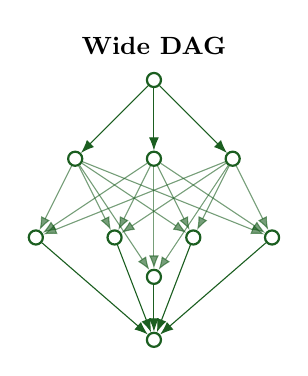
\begin{tikzpicture}[
      node/.style={circle,draw=WideColor,thick,fill=white,inner sep=1.8pt},
      edge/.style={-Latex,thin,draw=WideColor},
      >=Latex
    ]
    \node[node] (s) at (0,1.5) {};
    \node[node] (a1) at (-1,0.5) {};
    \node[node] (a2) at ( 0,0.5) {};
    \node[node] (a3) at ( 1,0.5) {};
    \node[node] (b1) at (-1.5,-0.5) {};
    \node[node] (b2) at (-0.5,-0.5) {};
    \node[node] (b3) at ( 0.5,-0.5) {};
    \node[node] (b4) at ( 1.5,-0.5) {};
    \node[node] (b5) at ( 0,-1.0)   {};
    \node[node] (t) at (0,-1.8) {};
    \foreach \x in {a1,a2,a3} \draw[edge] (s) -- (\x);
    \foreach \x in {a1,a2,a3}{
      \foreach \y in {b1,b2,b3,b4,b5}{
        \draw[edge,opacity=0.6] (\x) -- (\y);
      }
    }
    \foreach \x in {b1,b2,b3,b4,b5} \draw[edge] (\x) -- (t);
    \node[above=1mm of s] {\small \textbf{Wide DAG}};
  \end{tikzpicture}
  \hspace{1.6em}
  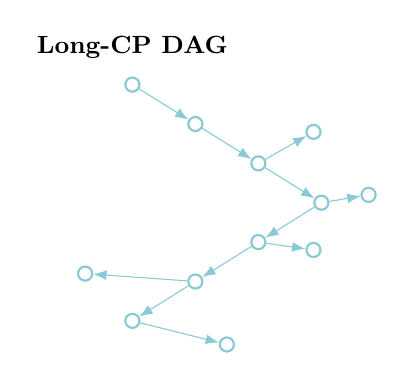
\begin{tikzpicture}[
      node/.style={circle,draw=longcpColor,thick,fill=white,inner sep=1.8pt},
      edge/.style={-Latex,thin,draw=longcpColor},
      >=Latex
    ]
    \node[node] (c0) at (-1.2,1.5) {};
    \node[node] (c1) at (-0.4,1.0) {};
    \node[node] (c2) at ( 0.4,0.5) {};
    \node[node] (c3) at ( 1.2,0.0) {};
    \node[node] (c4) at ( 0.4,-0.5) {};
    \node[node] (c5) at (-0.4,-1.0) {};
    \node[node] (c6) at (-1.2,-1.5) {};
    \node[node] (c7) at ( 0.0,-1.8) {};
    \node[node] (b2a) at ( 1.1,0.9)  {};
    \node[node] (b3a) at ( 1.8,0.1)  {};
    \node[node] (b4a) at ( 1.1,-0.6) {};
    \node[node] (b5a) at (-1.8,-0.9) {};
    \foreach \u/\v in {c0/c1,c1/c2,c2/c3,c3/c4,c4/c5,c5/c6,c6/c7}{
      \draw[edge] (\u) -- (\v);
    }
    \draw[edge] (c2) -- (b2a);
    \draw[edge] (c3) -- (b3a);
    \draw[edge] (c4) -- (b4a);
    \draw[edge] (c5) -- (b5a);
    \node[above=1mm of c0] {\small \textbf{Long‑CP DAG}};
  \end{tikzpicture}
  \caption{Schematic comparison of a Wide DAG (left, shallow with many parallel branches) and a Long‑CP DAG (right, deep dependency chain with limited side‑branch concurrency).}
  \label{fig:Wide_vs_longcp_tikz}
  \Description{Two DAG diagrams showing contrasting structures: a wide shallow DAG with high parallelism on the left, and a deep sequential DAG with limited parallelism on the right.}
\end{figure}

Figure~\ref{fig:search_space_landscape} shows how workflow structure changes the scheduling problem. Wide DAGs create a rugged landscape with shallow valleys everywhere. When many tasks are ready at once, there are countless ways to assign them to VMs. A small change in the assignment can cause energy consumption to jump around unpredictably.

LongCP DAGs produce a different landscape entirely. Fewer valleys, but deeper ones. The critical path constrains most decisions because dependency chains force a specific order. There's little room to explore alternatives. The main freedom is placing short side branches, which creates a few isolated basins instead of a chaotic surface.

\begin{figure}[htbp]
    \centering
    \includegraphics[width=0.8\columnwidth]{figs/3d_energy.png}
    \caption{Fitness landscape of the scheduling search space. We exhaustively enumerate all feasible action sequences for a small scenario and project them onto a 2D plane using a Hilbert curve. The Z-axis shows energy consumption (lower is better). Left: LongCP DAG. Right: Wide DAG.}
    \label{fig:search_space_landscape}
    \Description{3D visualization showing energy landscapes for two different DAG types, with LongCP showing deeper isolated valleys and Wide showing a more rugged surface.}
\end{figure}

With these distinctions, we address Q1 and Q2 through four host-configuration regimes (AL, NA, HS, HP) in our queue-free setting.

\subsubsection{Queue-Free Regime}
\label{sec:queue_free_shared}

Across all four regimes we assume a \emph{queue-free}, single-workflow environment. A cluster of $V$ virtual machines (VMs) executes a single DAG workflow. Time is continuous and tasks are non-migratable once assigned to a VM.

The dataset generator enforces queue-freedom: for each DAG we scale task memory and CPU requirements so that the peak-width layer fits within aggregate cluster capacity.

\subsubsection{Queue-Free, Homogeneous-Speed Regime}
\label{sec:queue_free_homogeneous_speed}

In the homogeneous-speed regime, all VMs process work at the same rate $s$ (e.g., MIPS). Because speeds are identical and the instance is queue-free, any non-pathological schedule that keeps critical-path tasks busy attains the same makespan $T^\star = L_{\mathrm{CP}} / s$.

We focus on power-heterogeneous but speed-homogeneous hosts. At approximately fixed makespan, the only remaining degree of freedom is which VMs are active and for how long. This means the policy can only shape active energy by controlling VM power profiles.

\subsubsection{Queue-Free, Homogeneous-Power Regime}
\label{sec:queue_free_homogeneous_power}

In the homogeneous-power regime, all VMs share the same active power $P^{\mathrm{act}}$ but differ in speed $s(v)$. Active energy is approximated as $E \approx \int P^{\mathrm{act}}\,dt$. For a fixed task workload, this makes energy largely insensitive to speed, while makespan still depends on $s(v)$ through $\tau = L/s(v)$.

The effective objective becomes primarily time-dominated: faster machines shorten makespan, but active energy remains approximately unchanged across VM choices since $P^{\mathrm{act}}$ is constant.

\subsubsection{Queue Free, Heterogeneous Aligned Regime}
\label{sec:queue_free_heterogeneous_aligned}

In the heterogeneous aligned regime, speed and energy efficiency move in the same direction. Faster machines are also more power efficient for the same amount of work. Moving a task to a faster VM therefore tends to reduce both completion time and total energy, so the two objectives are mostly aligned.

\subsubsection{Queue Free, Heterogeneous Non Aligned Regime}
\label{sec:queue_free_heterogeneous_nonaligned}

In the heterogeneous non aligned regime, we break this link between speed and efficiency. Some VMs are fast but energy hungry, while others are slow but energy cheap. Higher speed does not imply lower energy per unit work, and in some cases it can be strictly worse.

This creates real conflicts between local choices. A faster VM may reduce completion time but increase total energy, while a slower and more efficient VM may save energy at the cost of longer makespan.

\begin{figure}[htbp]
    \centering
    \includegraphics[width=0.6\columnwidth]{figs/host_regime_compass.png}
    \caption{Speed--power host regimes. Illustration of the four queue-free host regimes studied in this paper.}
    \label{fig:host_regime_compass}
    \Description{Diagram showing four different host regime configurations based on speed and power characteristics.}
\end{figure}

\section{Model Architecture}
\label{sec:architecture}

Our scheduler is a deep actor--critic architecture built around a shared graph neural network (GNN) backbone that embeds both workflow tasks and virtual machines (VMs). Figure~\ref{fig:gnn_architecture} summarizes the deep reinforcement learning architecture used throughout this work.

\begin{figure*}[htbp]
    \centering
    \includegraphics[width=\linewidth]{figs/gnn_actor_critic_architecture.png}
    \caption{Overview of the proposed GIN-based actor--critic scheduler architecture.}
    \label{fig:gnn_architecture}
    \Description{Architecture diagram showing the GNN-based actor-critic model with task and VM encoders, GIN layers, and policy/value heads.}
\end{figure*}

\paragraph{Input representation.}
At each decision step the environment provides a structured observation encoding the current workflow DAG and the VM pool. Tasks are represented by: (i) scheduled/ready flags, (ii) remaining work and completion time, (iii) CPU and memory requirements. VMs are represented by: (i) completion times and current utilization, (ii) speed, core count and available cores, (iii) memory capacity and free memory, (iv) host idle and peak power.

\paragraph{Task and VM encoders.}
We map raw task and VM features into a common latent space using two separate multi-layer perceptrons (MLPs). The task encoder consumes a 6-dimensional feature vector and outputs a $d$-dimensional embedding. The VM encoder consumes a 12-dimensional feature vector and outputs an embedding in the same space.

\paragraph{GIN backbone.}
We concatenate the encoded task and VM nodes into a single set and process them using a three-layer Graph Isomorphism Network (GIN) \cite{xu2019how} with hidden dimension $h$. The edges capture both task–VM compatibility links and task–task dependencies.

\paragraph{Actor and critic heads.}
After GIN message passing, we extract task and VM embeddings and use them in two separate heads. The actor computes logits for each feasible (task, VM) pair and applies a softmax to produce a categorical distribution. The critic aggregates all embeddings via global pooling and outputs a scalar state value estimate.

\section{Experimental Methodology}
\label{sec:exp_methodology}

\subsection{Training Setup}

We train separate specialist policies for Wide and LongCP DAG families using Proximal Policy Optimization (PPO). Each specialist is trained on 100 randomly generated workflows from its respective family across all four host regimes (HS, HP, AL, NA).

Training hyperparameters: learning rate $3 \times 10^{-4}$, batch size 2048, 10 PPO epochs per batch, clip parameter 0.2, entropy coefficient 0.01, value loss coefficient 0.5, discount factor $\gamma = 0.99$.

\subsection{Evaluation Protocol}

We evaluate each trained specialist on held-out test sets of 100 workflows from both Wide and LongCP families, across all four host regimes. This gives us a $2 \times 2 \times 4$ evaluation matrix: 2 specialists $\times$ 2 test families $\times$ 4 regimes.

For each configuration, we measure:
\begin{itemize}
\item Makespan (completion time)
\item Active energy consumption
\item Total energy (active + idle)
\item Pareto dominance metrics
\end{itemize}

We compare learned policies against classical heuristics: HEFT, CPOP, Earliest Completion Time (ECT), and Min-Min.

\subsection{Key Findings}

\subsubsection{Q1: Joint Influence of Structure and Host Configuration}

Our results show that DAG topology fundamentally shapes the policy's learned priorities, even under a fixed energy–makespan objective. Agents trained on different topologies implicitly attend to different structural and resource features.

In the Homogeneous Speed (HS) regime, where makespan is largely fixed by critical path length, the Wide specialist learns to minimize energy by carefully selecting low-power VMs. The LongCP specialist, facing limited parallelism, focuses on keeping the critical path busy and shows less sensitivity to power differences.

In the Homogeneous Power (HP) regime, where energy is approximately constant, both specialists converge to time-minimization strategies. However, the LongCP specialist achieves lower makespan because its training distribution emphasized critical path optimization.

In the Aligned (AL) regime, where speed and efficiency move together, both specialists perform well but the LongCP specialist shows a slight advantage because the problem reduces to a simpler time-dominated objective that matches its training bias.

In the Non-Aligned (NA) regime, where speed and efficiency conflict, the two specialists develop complementary strengths. The Wide specialist achieves lower makespan by exploiting fast VMs, while the LongCP specialist achieves lower energy by preferring efficient VMs. This divergence occurs because the training state distributions differ: Wide DAGs expose many parallel choices where speed matters, while LongCP DAGs expose sequential bottlenecks where efficiency matters.

\subsubsection{Q2: Cross-Structure Generalization}

Cross-structure generalization varies dramatically across host configurations. In HS and HP regimes, where one objective dominates, specialists can partially transfer across structures. In AL regime, the LongCP specialist generalizes reasonably well to Wide DAGs because the objectives are aligned. In NA regime, cross-structure generalization fails systematically: the Wide specialist performs poorly on LongCP DAGs (high energy) and the LongCP specialist performs poorly on Wide DAGs (high makespan).

These failures are not random. They concentrate in specific out-of-distribution combinations where the training distribution's structural properties (parallelism, critical path length, ready set sizes) differ sharply from the test distribution.

\subsubsection{Q3: When Heuristics Suffice vs. When Specialists Are Needed}

In HS and HP regimes, simple heuristics often match or exceed learned policies. In HS, a power-minimizing heuristic suffices. In HP, a makespan-minimizing heuristic suffices.

In AL regime, heuristics perform well in simple cases, but the LongCP specialist shows advantages as problem complexity increases.

In NA regime, neither heuristics nor a single specialist dominates. The Wide specialist achieves lower makespan, while the LongCP specialist achieves lower energy. A practical approach is regime-aware routing: classify the environment by computing variance of speeds, variance of powers, and their correlation, then route to the appropriate expert or heuristic.

\section{Interpretability Analysis}

To understand why cross-structure generalization fails in the NA regime, we analyze the state space geometry and policy behavior.

Figure~\ref{fig:state-visitation-structure} shows state visitation distributions for Wide and LongCP specialists during training. The LongCP specialist concentrates density in low-parallelism, moderate-energy regions because dependency chains limit ready set sizes. The Wide specialist shifts density toward high-parallelism, higher-energy regions because parallel structure enables many simultaneous task-VM assignments.

Both agents optimize the same objective function, but DAG structure changes which states are reachable and frequently visited. Long critical paths compress the feasible manifold toward low parallelism, so the policy places more mass in regions where energy-reducing choices matter. Wide DAGs expand the feasible trajectory set in parallel directions, so the policy shifts toward states where time-reducing choices are available.

This explains the cross-evaluation results: when the LongCP specialist is tested on Wide configurations, it still tries to minimize energy. When the Wide specialist is tested on LongCP configurations, it still tries to minimize makespan. Neither strategy is wrong, they just learned different priorities from different training distributions.

\section{Conclusion}

The challenge of efficiently scheduling complex, dependency-driven workflows in modern cloud environments requires balancing completion time (makespan) against energy consumption. Deep RL schedulers with GNN backbones are a promising alternative to classical heuristics, but their robustness and generalization across workflow structures and hardware regimes remain open questions.

In this work, we addressed this by constructing a controlled benchmark that factorizes the problem into two contrasting DAG topologies (Wide and LongCP) and four host regimes (HS, HP, AL, NA). By training specialized agents and subjecting them to systematic cross-structure and cross-regime evaluation, we have successfully answered the three research questions posed in Section~\ref{sec:introduction}.

Our results show that DAG topology fundamentally shapes the policy's learned priorities, even under a fixed energy–makespan objective. Generalization failures are structured rather than random: performance drops concentrate in specific out-of-distribution combinations of topology and host regime, with the NA configuration exposing the sharpest trade-off between speed and energy. These findings highlight the brittleness of a single, monolithic deep RL scheduler.

Motivated by this, we argued for a structure- and regime-aware routing approach: instead of enforcing a universally robust agent, first characterize the environment and then route jobs to specialized policies or heuristics that are best suited to that region of the space.

This research opens several avenues for future investigation. The most immediate is the formalization and implementation of the proposed routing mechanism. Furthermore, future work should explore domain-agnostic training techniques through meta-learning or domain randomization approaches. Finally, extending this analysis to a queue-based setting with multiple concurrent workflows is essential for real-world deployment.

%%
%% The acknowledgments section is defined using the "acks" environment
%% (and NOT an unnumbered section). This ensures the proper
%% identification of the section in the article metadata, and the
%% consistent spelling of the heading.
\begin{acks}
The authors would like to thank the reviewers for their valuable feedback and suggestions.
\end{acks}

%%
%% The next two lines define the bibliography style to be used, and
%% the bibliography file.
\bibliographystyle{ACM-Reference-Format}
\bibliography{tmlr}

\end{document}
